% v5 pilot results and candidate-aligned flavour-tagging variables.
\documentclass[aspectratio=169,10pt]{beamer}
\usetheme{Boadilla}
\usecolortheme{default}
\usepackage{booktabs}
\usepackage{graphicx}
\usepackage{amsmath}
\usepackage{array}
\usepackage{url}
\definecolor{navy}{HTML}{17365D}
\definecolor{orange}{HTML}{D97931}
\setbeamercolor{structure}{fg=navy}
\setbeamercolor{frametitle}{fg=navy}
\setbeamercolor{block title}{fg=white,bg=navy}
\setbeamercolor{block body}{bg=navy!5}
\setbeamertemplate{navigation symbols}{}
\setbeamertemplate{footline}[frame number]
\graphicspath{{figures/}}
\newcommand{\tinyref}[1]{\vfill\par{\tiny\color{gray}#1}}

\title[v5 flavour-tagging pilot]{v5 event-jet flavour tagging}
\subtitle{Signal pilot, opposite-jet Z-flavour check, and saved candidate variables}
\author{FCC-ee analysis review}
\date{6 October 2026}

\begin{document}
\begin{frame}
  \titlepage
  \vspace{-0.4cm}
  \begin{center}\small Diagnostic studies only; no tag cut or BDT has been adopted.\end{center}
\end{frame}

\begin{frame}{Question and study scope}
\begin{block}{Physics question}
Can the flavour of the event jet opposite a reconstructed $\Lambda_b\to\Lambda^0\gamma$ candidate help distinguish signal-like $Z\to b\bar b$ events from selected $Z\to s\bar s$ and $Z\to c\bar c$ candidates?
\end{block}
\begin{itemize}
  \item Run the existing reconstructed candidate selection and attach pretrained Weaver scores to two exclusive-$ee$-$k_t$ jets.
  \item Associate each candidate to its nearest jet by direction; call the other jet the opposite jet.
  \item Keep truth as an evaluation label. No FT score is a Stage 1 selection.
\end{itemize}
\begin{alertblock}{Scope}
The pilot is unweighted and low statistics. It tests saved variables and a separation hypothesis; it does not estimate inclusive rejection or expected yields.
\end{alertblock}
\tinyref{Implementation: analysis/studies/lb2lambda\_gamma\_reco\_v5.py. Study definitions: docs/STAGE1\_V5\_FLAVTAG\_VARIABLES.md.}
\end{frame}

\begin{frame}{Processing and selections}
\small
\begin{enumerate}
  \item Build reconstructed $p\pi$ and photon candidates with the v5 reconstruction config; include both charge conjugates.
  \item Keep the established fitted-$\Lambda^0$ mass and vertex requirements. Apply the $E(\Lambda_b)\geq10.5$ GeV event gate after candidate building and before truth annotation and tagger inference.
  \item Cluster all reconstructed particles into two event jets; supply the reconstructed PV to Weaver and save class scores per jet.
  \item Copy the nearest-jet and other-jet scores onto each candidate; flatten to one row per candidate with event and candidate keys.
\end{enumerate}
\begin{block}{Known modelling caveats}
The pretrained model used MC PV inputs upstream; this study supplies a reconstructed PV. Candidate daughters are not removed before jet clustering. Both choices need calibration checks.
\end{block}
\tinyref{Config: config/lb\_reco\_v5\_training.json. Shared offline region in reports: fitted $|m(p\pi)-1.115683|\leq12.5$ MeV and $E(\Lambda_b)\geq10.5$ GeV.}
\end{frame}

\begin{frame}{Signal pilot: the variables survive normal processing}
\begin{columns}[T]
\begin{column}{0.52\textwidth}
\begin{itemize}
  \item 1,000 Physics input events; 584 candidate-bearing output events.
  \item 627 flattened candidate rows; 572 truth-matched signal rows.
  \item Shared offline region: 612 candidates, including the 572 matched rows.
  \item All ten B/C/S/Q/G candidate-aligned score columns are present with no nulls in that region.
\end{itemize}
\end{column}
\begin{column}{0.44\textwidth}
\begin{block}{Other-jet b-score retention}
\centering
\begin{tabular}{lr}
\toprule
Threshold & Matched signal retained\\
\midrule
$\geq0.50$ & 91.4\%\\
$\geq0.80$ & 88.5\%\\
$\geq0.90$ & 85.3\%\\
$\geq0.95$ & 80.1\%\\
$\geq0.99$ & 40.7\%\\
\bottomrule
\end{tabular}
\end{block}
\end{column}
\end{columns}
\begin{alertblock}{Interpretation}
These are signal-only raw score efficiencies. They measure no background rejection and are not cut recommendations.
\end{alertblock}
\tinyref{Signal pilot report: docs/STAGE1\_V5\_FLAVTAG\_SIGNAL\_PILOT\_2026-10-05.md.}
\end{frame}

\begin{frame}{Six-file Z-flavour pilot: opposite jet is flavour-sensitive}
\small
\begin{columns}[T]
\begin{column}{0.47\textwidth}
\begin{tabular}{lrrr}
\toprule
Sample & Inputs & Rows in region & Events\\
\midrule
Zbb & 6,000 & 16 & 16\\
Zcc & 6,000 & 29 & 26\\
Zss & 6,000 & 39 & 36\\
\bottomrule
\end{tabular}
\vspace{0.3cm}

Largest other-jet B/C/S score predicted the generated sample flavour for 74/78 selected events.
\end{column}
\begin{column}{0.50\textwidth}
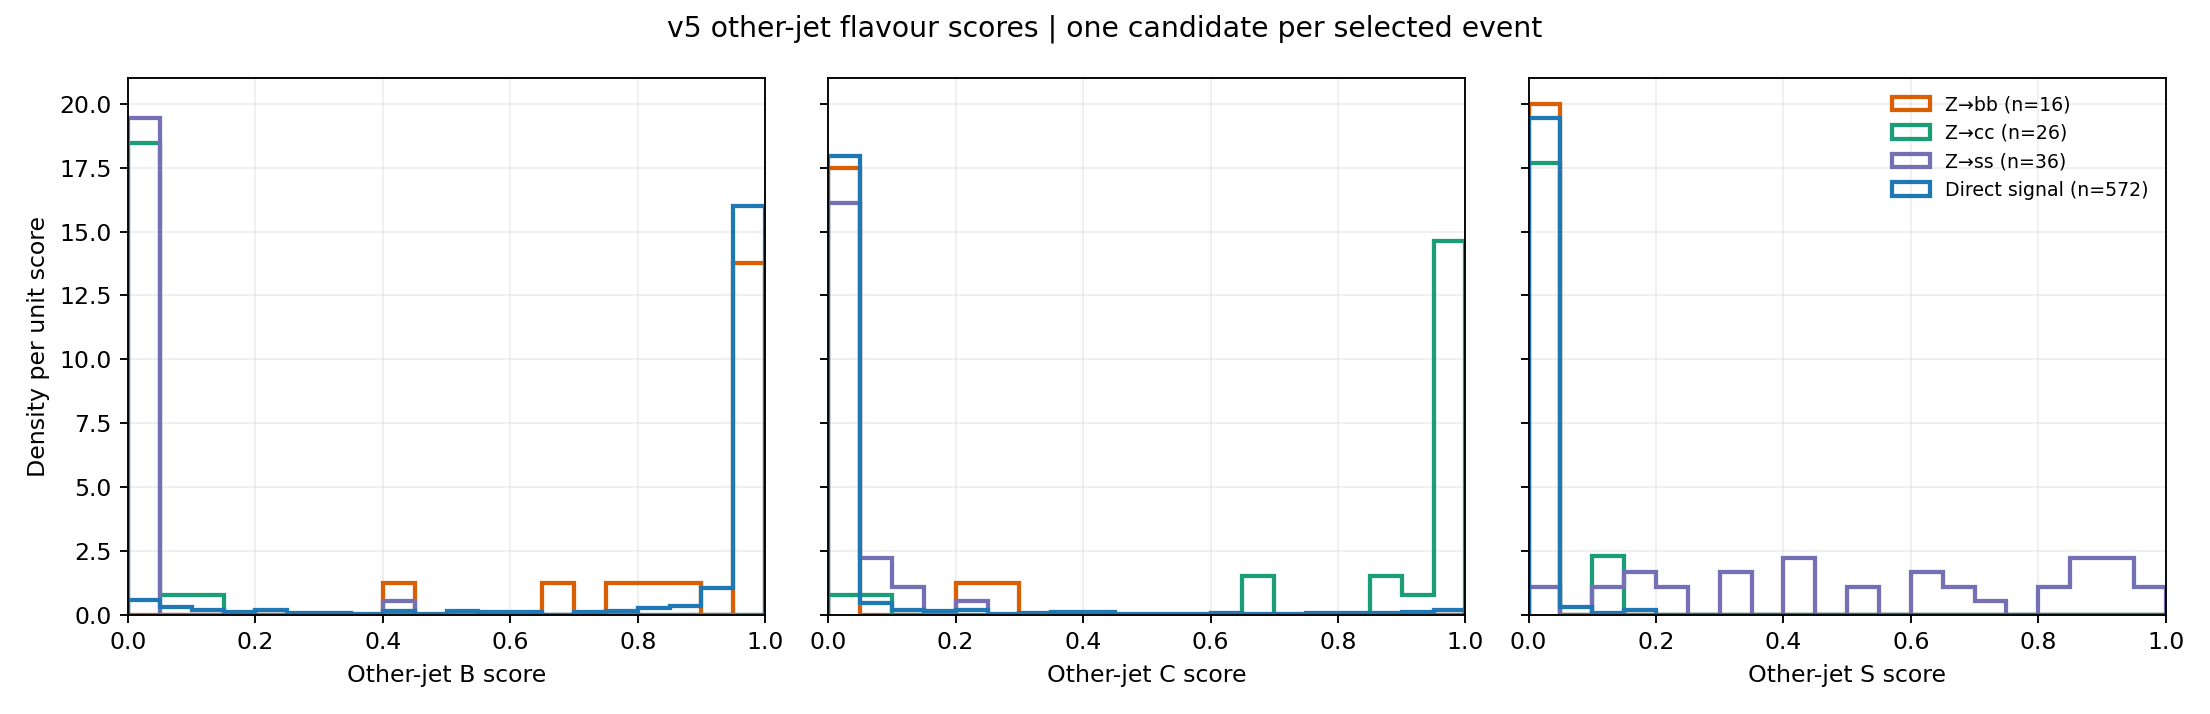
\includegraphics[width=\textwidth]{otherjet_bcs_scores.png}
\end{column}
\end{columns}
\begin{block}{Raw other-jet $b\geq0.8$ diagnostic}
Direct signal: 506/572 (88.5\%); Zbb: 13/16; Zcc: 0/26; Zss: 0/36.
\end{block}
\tinyref{Curves are unit-normalized score shapes, not event yields. Six files and first 1,000 entries per file; no cross-section weights. See docs/STAGE1\_V5\_ZFLAVOUR\_PILOT\_2026-10-06.md.}
\end{frame}

\begin{frame}{Candidate-aligned flavour-tag scores}
\scriptsize
\begin{tabular}{p{0.10\textwidth}p{0.60\textwidth}p{0.25\textwidth}}
\toprule
Class $X$ & Exact candidate branches & Meaning\\
\midrule
B & \parbox[t]{0.60\textwidth}{\path{lb_flavtag_v5_recojet_isB_flavtag_v5_associated}\\\path{lb_flavtag_v5_recojet_isB_flavtag_v5_otherjet_max}} & Candidate-side jet b score; other-jet b score.\\
C & \parbox[t]{0.60\textwidth}{\path{lb_flavtag_v5_recojet_isC_flavtag_v5_associated}\\\path{lb_flavtag_v5_recojet_isC_flavtag_v5_otherjet_max}} & Candidate-side jet c score; other-jet c score.\\
S & \parbox[t]{0.60\textwidth}{\path{lb_flavtag_v5_recojet_isS_flavtag_v5_associated}\\\path{lb_flavtag_v5_recojet_isS_flavtag_v5_otherjet_max}} & Candidate-side jet s score; other-jet s score.\\
Q & \parbox[t]{0.60\textwidth}{\path{lb_flavtag_v5_recojet_isQ_flavtag_v5_associated}\\\path{lb_flavtag_v5_recojet_isQ_flavtag_v5_otherjet_max}} & Candidate-side jet light-quark score; other-jet light-quark score.\\
G & \parbox[t]{0.60\textwidth}{\path{lb_flavtag_v5_recojet_isG_flavtag_v5_associated}\\\path{lb_flavtag_v5_recojet_isG_flavtag_v5_otherjet_max}} & Candidate-side jet gluon score; other-jet gluon score.\\
\bottomrule
\end{tabular}
\vspace{0.2cm}

\texttt{associated} means the jet nearest the reconstructed candidate direction. \texttt{otherjet\_max} is the maximum score among the remaining jets (the opposite jet for the default two-jet setup). Missing association/score is encoded as $-1$.

\tinyref{Per-jet vectors are saved; the proposed BDT uses six B/C/S scores.}
\end{frame}

\begin{frame}{What is stored per candidate beyond the ten FT scores?}
\small
\begin{tabular}{p{0.22\textwidth}p{0.70\textwidth}}
\toprule
Candidate family & Saved information\\
\midrule
Identity and truth labels & \texttt{event\_entry}, candidate slot/multiplicity, charge sign, reconstructed-to-MC match and ancestry labels. Truth is attached after candidate building.\\
Candidate kinematics & Four-momenta and masses for proton, pion, fitted $\Lambda^0$, photon and $\Lambda_b$; helicity angle and thrust/hemisphere observables.\\
Vertex and displacement & Fitted PV/SV quantities, vertex quality, daughter $d_0$ significances, $\Lambda^0$ flight and impact-parameter observables.\\
Event activity & Photon- and $\Lambda^0$-centred isolation, recoil/balance and photon-partner diagnostics; these remain available independently of the FT scores.\\
Flavour tagging & Ten candidate-aligned B/C/S/Q/G score columns shown on the preceding slide, plus event-level jet vectors and kinematics.\\
\bottomrule
\end{tabular}
\vspace{0.3cm}
\begin{alertblock}{Candidate granularity}
The Stage 1 ROOT tuple stores candidate vectors per event. Flattening produces one row per candidate and retains event keys and candidate multiplicity.
\end{alertblock}
\tinyref{Detailed branch definitions: docs/STAGE1\_V5\_FLAVTAG\_VARIABLES.md.}
\end{frame}

\begin{frame}{Limits and next decision}
\begin{itemize}
  \item Only 78 selected Zbb/Zcc/Zss events survive the pilot region; 0/36 Zss events passing the b-score cut is not evidence of zero inclusive Zss background.
  \item Opposite b tagging also retains 13/16 selected Zbb candidates, as expected for a signal produced in $Z\to b\bar b$.
  \item No production weights were used; file IDs and entry ranges are a bounded pilot, not an inclusive mixture.
  \item Weaver inputs use reconstructed PV and include candidate daughters in the clustered jets; calibrate both effects.
\end{itemize}
\begin{block}{Recommended next comparison}
Train a combined BDT with the six B/C/S associated/other-jet scores plus the frozen offline feature set. Evaluate on independent, larger v5 Zbb/Zcc/Zss samples at matched signal efficiency, keeping direct signal, wrong combinations, and each background separate.
\end{block}
\centering The PI decides whether a later threshold or model becomes a selection scenario.
\tinyref{No v5 Condor jobs have been submitted. The Z-flavour Condor checks were check-only.}
\end{frame}
\end{document}
